\section{Experiment: Indirect Plasticity}

\begin{frame}{Indirect Plasticity: Conditional Initial State}
\begin{figure}
  \centering
  \begin{subfigure}[b]{\textwidth}
    \centering
    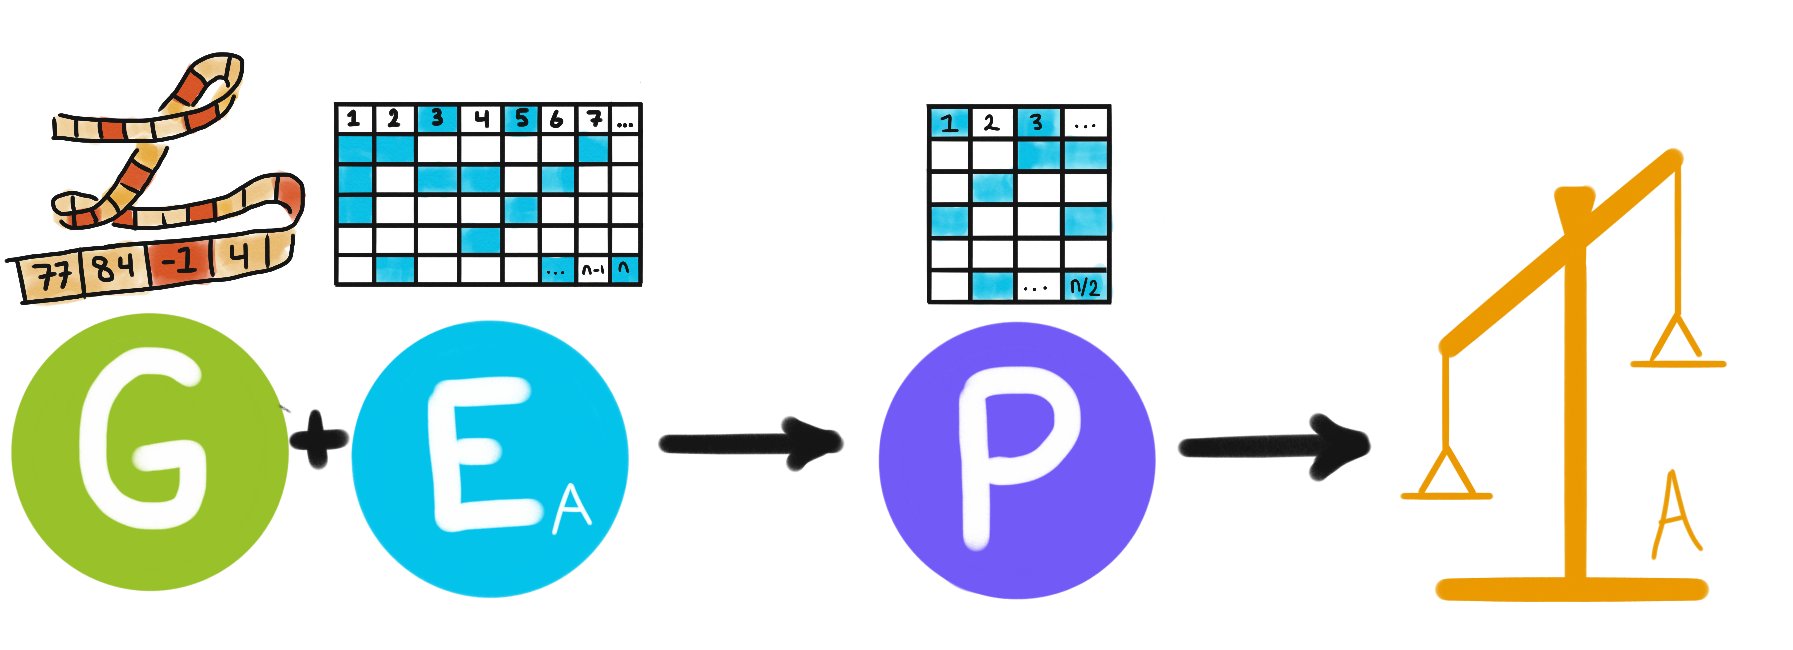
\includegraphics[width=0.4\textwidth]{img/indirectschemeA} \\
    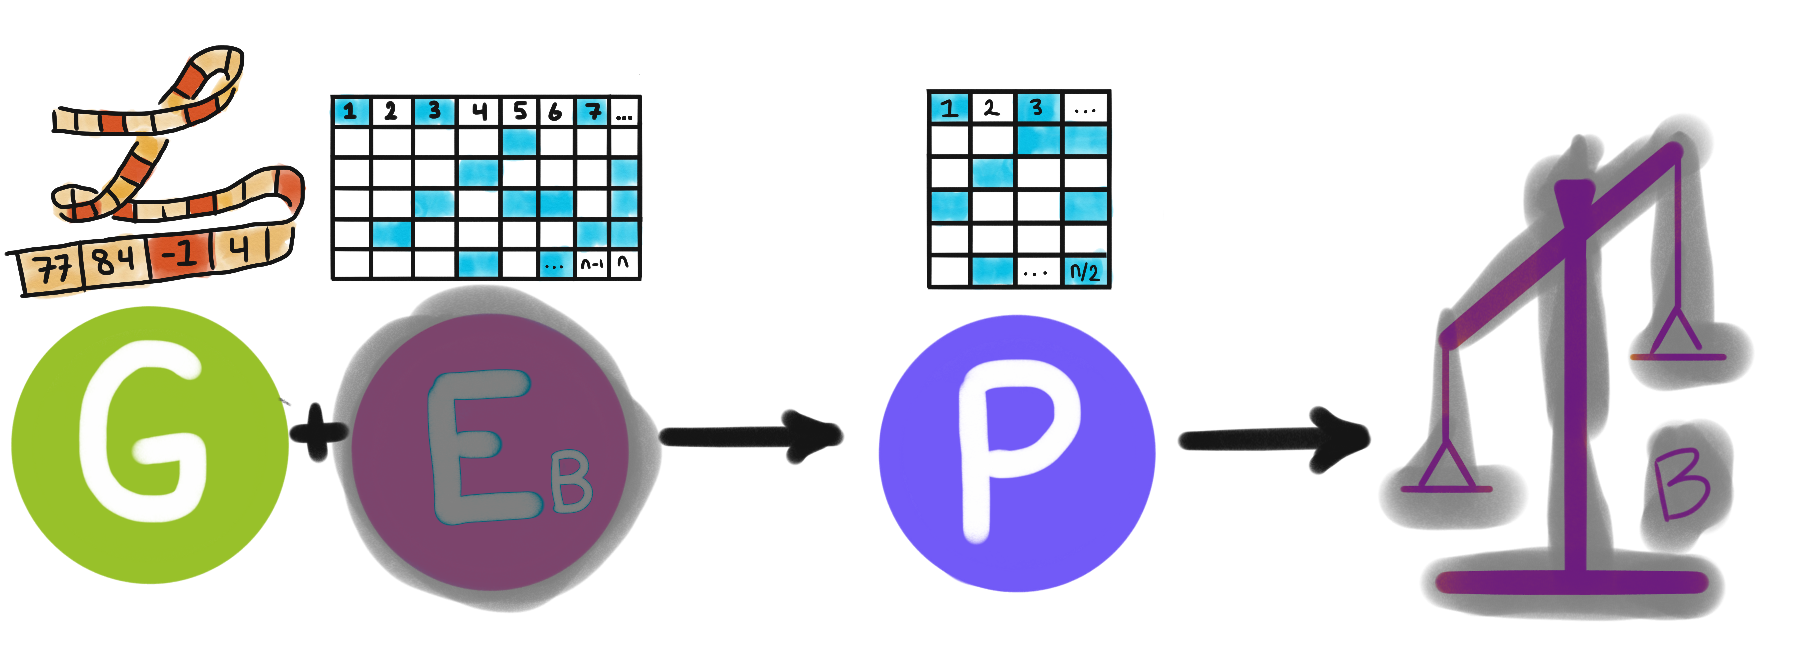
\includegraphics[width=0.4\textwidth]{img/indirectschemeB}
    \caption{experimental scheme}
    \label{subfig:directscheme}
  \end{subfigure}
  \hfill
  \begin{subfigure}[b]{\textwidth}
    \centering
    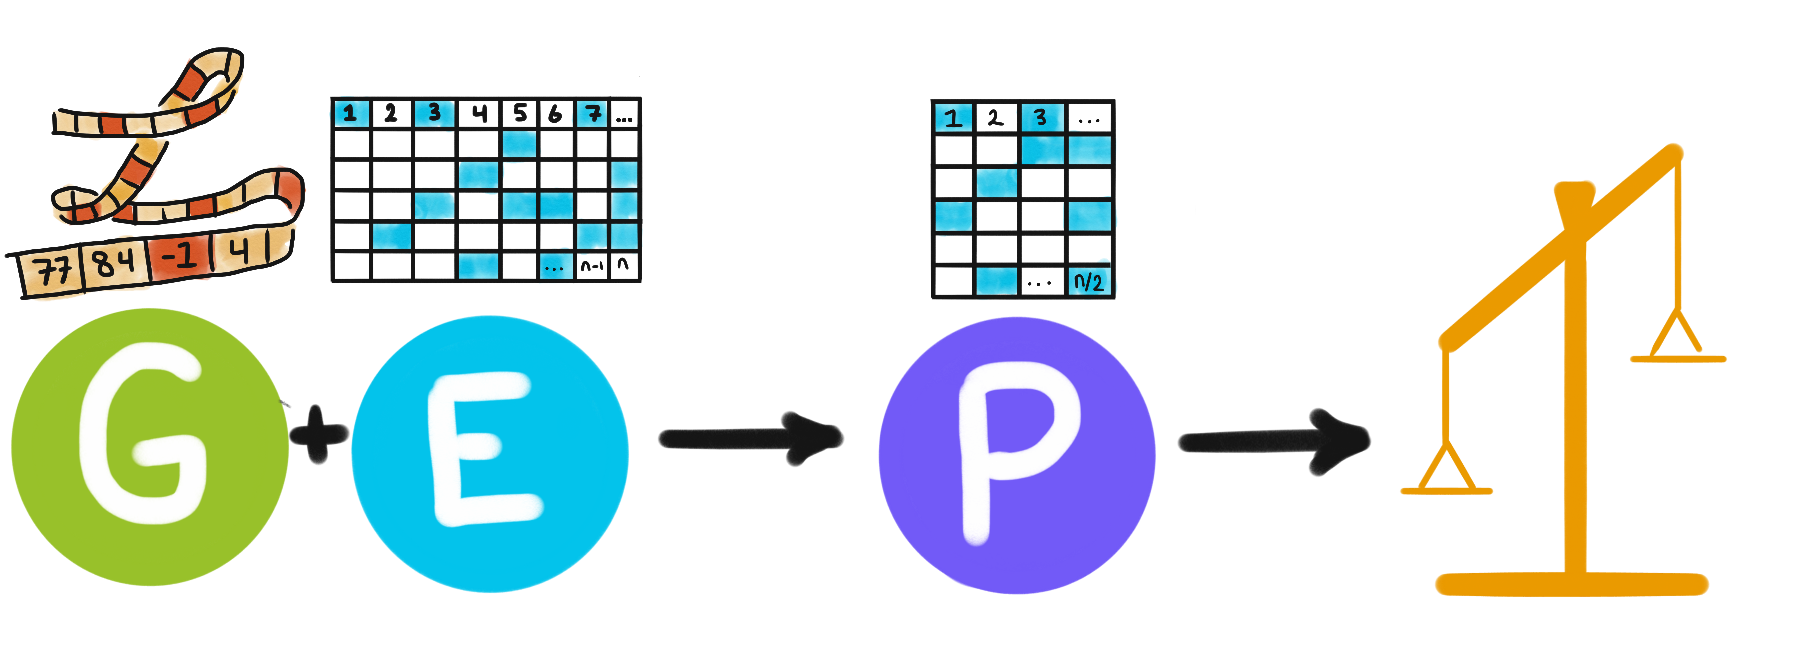
\includegraphics[width=0.4\textwidth]{img/modelscheme}
    \caption{control scheme}
     \label{subfig:controlscheme}
  \end{subfigure}
  \captionsetup{singlelinecheck=off,justification=raggedright}
  \caption{A comparison of the control and experimental schemes employed to investigate the relationship between indirect plasticity and evolvability.}
  \label{fig:direct_plasticity_scheme}
\end{figure}
\end{frame}

\begin{frame}{Evidence for Indirect Plasticity}
\begin{figure}
    \centering
    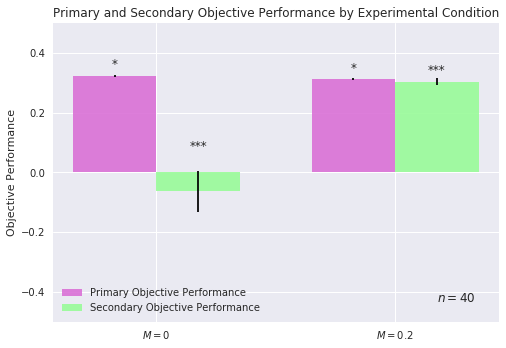
\includegraphics[width=0.8\textwidth]{img/primary_secondary_performance}
 	\captionsetup{singlelinecheck=off,justification=raggedright}
  	\caption{Comparison of objective performances of champions evolved with only primary condition/objective pair versus with both primary and secondary condition/objective pairs.}
    \label{fig:ev_w0}
\end{figure}
\end{frame}

\begin{frame}{Evolvability Visualization $W=0$}
\begin{figure}
    \centering
    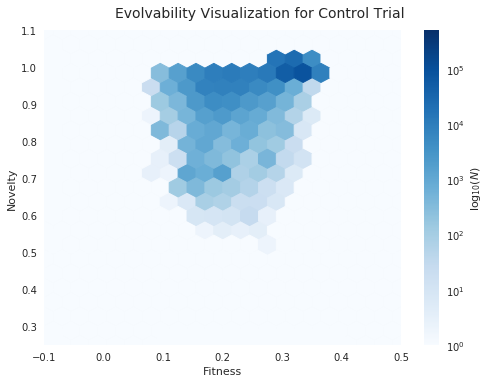
\includegraphics[width=0.8\textwidth]{img/ev_w0}
 	\captionsetup{singlelinecheck=off,justification=raggedright}
  	\caption{Evolvability visualization of champions evolved with only a primary condition/objective pair.}
    \label{fig:ev_w0}
\end{figure}
\end{frame}

\begin{frame}{Evolvability Visualization $W=0.2$}
\begin{figure}
    \centering
    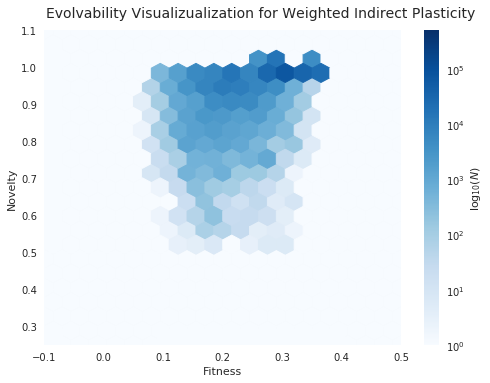
\includegraphics[width=0.8\textwidth]{img/ev_w0_2}
 	\captionsetup{singlelinecheck=off,justification=raggedright}
  	\caption{Evolvability visualization of champions evolved with primary and secondary condition/objective pairs.}
    \label{fig:es_w0_2}
\end{figure}
\end{frame}

\begin{frame}{Mutational Outcome Frequencies}
\begin{figure}
    \centering
    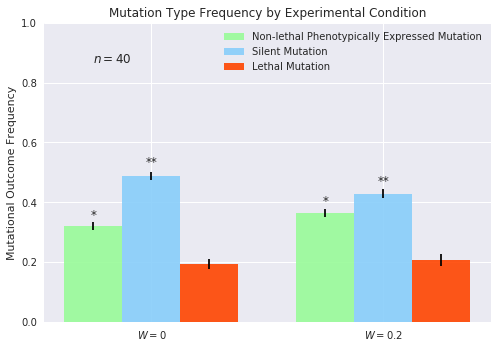
\includegraphics[width=0.8\textwidth]{img/mutation_type_indirect}
 	\captionsetup{singlelinecheck=off,justification=raggedright}
  	\caption{Comparison of mutational outcome frequencies for champions evolved with only primary condition/objective pair versus with both primary and secondary condition/objective pairs.}
    \label{fig:mutation_type_indirect}
\end{figure}
\end{frame}

\begin{frame}{Frequency of Useful Novelty}
 
 \begin{figure}
 \begin{subfigure}[b]{0.5\textwidth}
    \centering
    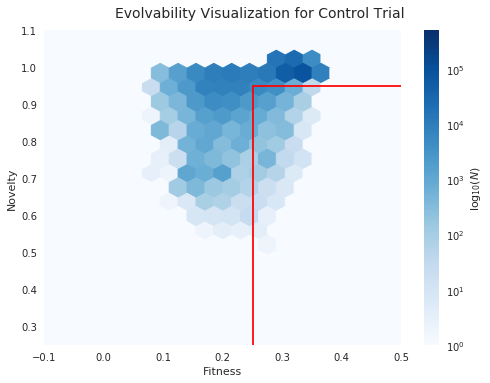
\includegraphics[width=\textwidth]{img/ev_w0_target}
    \caption{evolved with only primary condition/objective pair}
    \label{subfig:primary_only}
  \end{subfigure}%
    \begin{subfigure}[b]{0.5\textwidth}
    \centering
    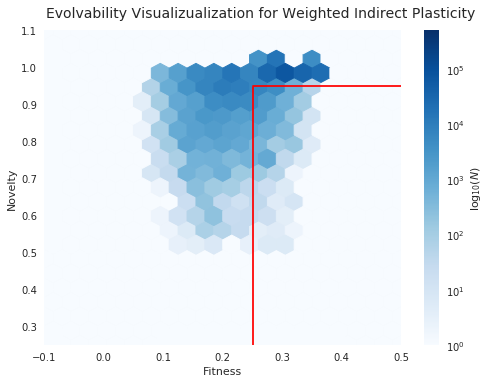
\includegraphics[width=\textwidth]{img/ev_w0_2_target}
    \caption{evolved with both primary and secondary condition/objective pairs}
    \label{subfig:primary_secondary}
  \end{subfigure}%

 	\captionsetup{singlelinecheck=off,justification=raggedright}
  	\caption{Comparison of evolvability visualizations with region corresponding to useful novelty highlighted.}
    \label{fig:freq_useful_novelty}
\end{figure}
\end{frame}

\begin{frame}{Indirect Plasticity Results: Summary}
\begin{itemize}
  \item indirect plasticity observed
  \item indirect plasticity increases sensitivity to mutation
  \item indirect plasticity may promote useful novelty 
\end{itemize}
\end{frame}